\documentclass[12pt]{ctexart}

% 包含必要的包
\usepackage[utf8]{inputenc}
\usepackage{amsmath, amssymb}  % 数学符号包
\usepackage{graphicx}  % 插入图片的包
\usepackage{hyperref}  % 生成超链接
\usepackage{fancyhdr}  % 页眉页脚设置
\usepackage{geometry}  % 页面设置
\usepackage{titlesec}  % 用于自定义 section 的格式
\usepackage{float}
\usepackage{listings}
\usepackage{xcolor}

\geometry{a4paper, margin=1in}

\titleformat{\section}[hang]{\normalfont\Large\bfseries}{\thesection}{1em}{}

\lstset{
    language=Python,
    basicstyle=\ttfamily\small,
    keywordstyle=\color{blue},
    stringstyle=\color{red},
    commentstyle=\color{green!50!black},
    numbers=left,
    numberstyle=\tiny\color{gray},
    frame=single,
    breaklines=true,
    backgroundcolor=\color{gray!10},
    showstringspaces=false,
    % captionpos=b % 让代码标题出现在代码下方
}

% Header and footer
\setlength{\headheight}{14.49998pt}
\addtolength{\topmargin}{-2.49998pt}

\pagestyle{fancy}
\fancyhf{}
\fancyhead[L]{《统计信号处理》实验报告}
% \fancyhead[M]{清华大学}
\fancyhead[R]{刘昱杉 2024214103}
\fancyfoot[C]{\thepage}



\begin{document}

\begin{titlepage}
    \begin{center}
        % Insert logo
        
\includegraphics[width=5cm]{tsinghua_logo.png}\\[4cm]  % 插入图标并设置下方间距
        {\Huge 实验三:图像分割实验} \\[4cm]
        {\large 刘昱杉  \ \  2024214103}\\[6cm]
        {\normalsize \today}\\[1cm]
        \vfill
        \text{注:本实验报告为单人独立完成}\\
        \text{关于本实验报告对应的源码及实验环境,详见\texttt{code}目录下\texttt{readme}}

    \end{center}
\end{titlepage}

\section*{图像自动分割算法}

\subsection*{算法原理}

阈值分割(Thresholding)是图像分割中最常见的基本方法之一。
根据灰度分布,将图像中像素划分为前景和背景两部分,前景可视为“目标”,背景为“非目标”。

对于实验中提供的血液显微图像而言,\textbf{细胞区域}与\textbf{背景}在灰度上存在一定差异,利用此方法进行初步分割。

通过选用\textbf{Otsu}算法,可以自动确定最佳阈值,将图像分割为前景和背景两部分。
Otsu算法通过自动求取一个全局的最佳分割阈值,使得前景像素与背景像素类内方差最小,从而避免人工手动阈值,效果最好。

此外,针对血液图像,进行\textbf{形态学处理},进一步提取细胞区域。
\begin{itemize}
    \item 开运算(Opening):先腐蚀后膨胀,主要用于去除前景中的小噪点。
    \item 闭运算(Closing):先膨胀后腐蚀,主要用于填充前景中的孔洞。
\end{itemize}

实验的算法流程如下:
\begin{itemize}
    \item 第一步,对原始图片进行平滑滤波,去除噪声干扰。
    \item 第二步,利用Otsu算法进行阈值分割,得到二值图像,细胞为前景(0,白色),背景为背景(255,黑色)。
    \item 第三步,进行形态学处理,提取细胞区域。
    \item 第四步,根据所提供的参考图片,将图片转换为三通道,并将背景替换浅绿色(0,128,0)。
    \item 第五步,通过对比分割后的图片与初始图片逐像素对比,比较自动分割算法的表现。
\end{itemize}

\subsection*{实验结果}

实验中,对于提供的血液显微图像,经过上述算法处理后,得到的各个步骤结果如下:

\begin{figure}[H]
    \centering
    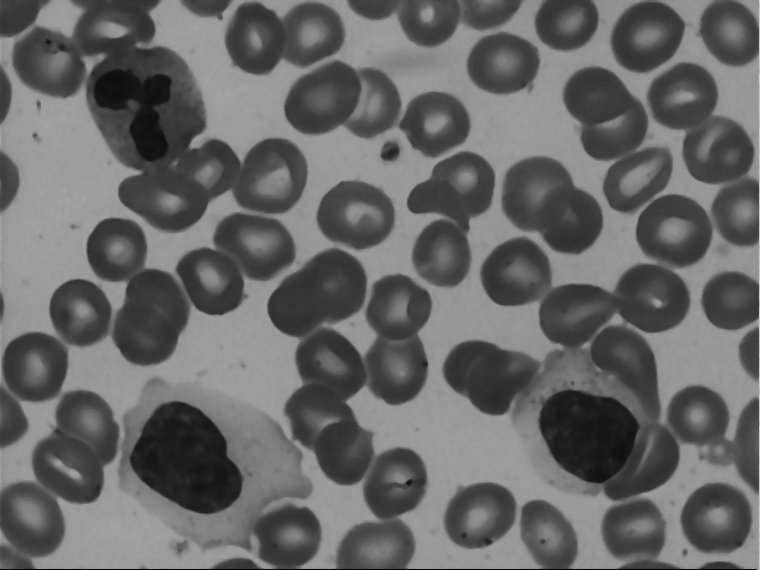
\includegraphics[width=0.7\textwidth]{image/gray_smooth.png}
    \caption{图平滑滤波结果}
\end{figure}

\begin{figure}[H]
    \centering
    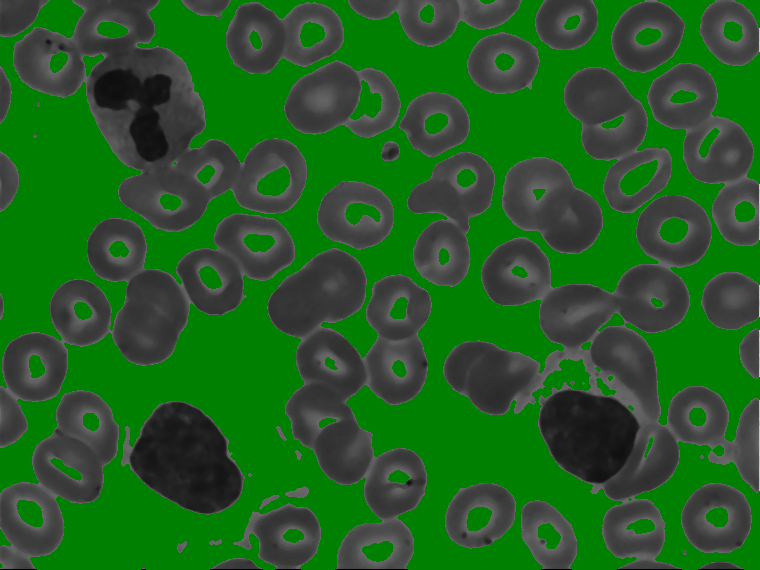
\includegraphics[width=0.7\textwidth]{image/gray_seg.png}
    \caption{Otsu算法分割与形态学处理结果}
\end{figure}

通过像素计算,得到与参考图片差异值为0,说明自动分割算法的表现较好。

\newpage

\section*{医学图像分割实验}

\subsection*{实验简介}

本实验旨在通过两种方法(传统的图像分割方法和基于深度学习的U-Net模型)对医学图像进行分割,并比较其性能。
实验数据来自ISBI 2012挑战赛的果蝇腹神经索切片图像数据。

本实验的主要目标包括:
\begin{itemize}
    \item 基于大津阈值法的医学图像分割
    \item 构建并训练基于U-Net的深度学习模型,完成医学图像分割任务
    \item 对比两种方法的性能,分析其优缺点
\end{itemize}

实验环境:
\begin{itemize}
    \item Python 3.8
    \item MindSpore 1.1.1
    \item ModelArts Platform
\end{itemize}

\subsection*{实验流程}

\subsubsection*{数据加载与可视化}
\begin{lstlisting}[language=Python]
    img_path = "./images/train/images"
    image= np.array([np.array(Image.open(os.path.join(img_path, name))) for name in os.listdir(img_path)])
    
    label_path = "./images/train/label"
    label= np.array([np.array(Image.open(os.path.join(label_path, name))) for name in os.listdir(label_path)])
    
\end{lstlisting}

\begin{figure}[H]
    \centering
    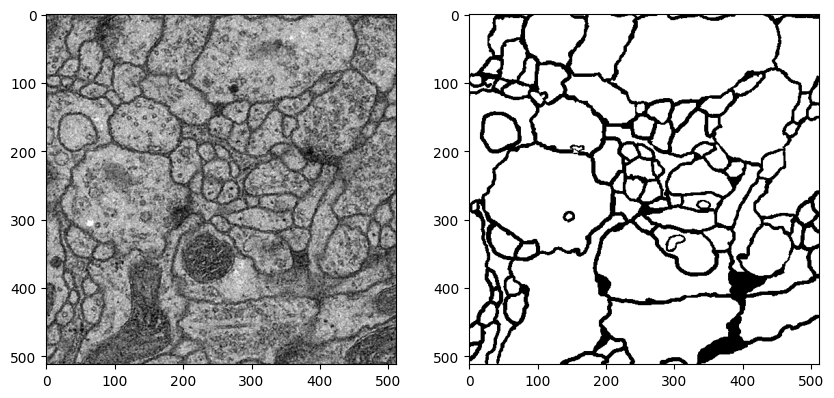
\includegraphics[width=0.7\textwidth]{image/output.png}
    \caption{初始数据}
\end{figure}

\subsubsection*{使用大津阈值法进行图像分割}

\begin{lstlisting}[language=Python]
    ret1, th1 = cv2.threshold(src=image[0], thresh=0, 
    maxval=255, type=cv2.THRESH_OTSU)
\end{lstlisting}


\textbf{结果分析:}
\begin{itemize}
    \item 大津阈值法对简单背景的分割效果较好,但对复杂的神经组织边界分割效果有限。
    \item 算法适合对比度明显的图像,不适用于复杂纹理背景。
\end{itemize}

\begin{figure}[H]
    \centering
    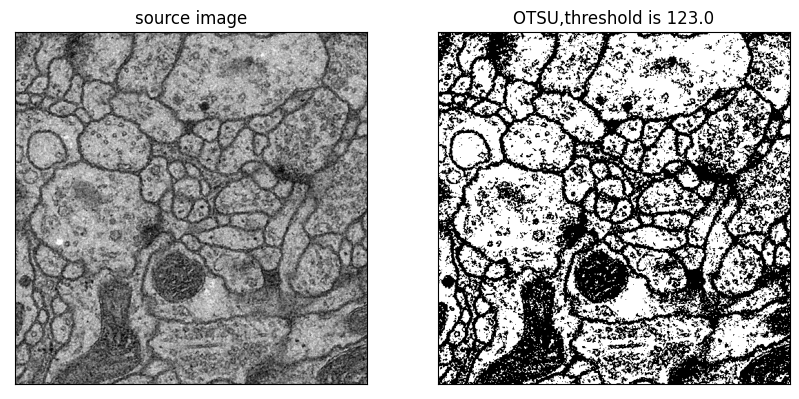
\includegraphics[width=0.7\textwidth]{image/1.png}
    \caption{大津阈值法分割结果}
\end{figure}


\subsubsection*{基于U-Net的深度学习方法}
\textbf{网络构建}
\newpage
\begin{lstlisting}[language=Python,caption={网络参数}]
    cfg_unet = {
        'name': 'Unet',
        'lr': 0.0001,
        'epochs': 400,
        'distribute_epochs': 1600,
        'batchsize': 16,
        'cross_valid_ind': 1,
        'num_classes': 2,
        'num_channels': 1,
        'keep_checkpoint_max': 10,
        'weight_decay': 0.0005,
        'loss_scale': 1024.0,
        'FixedLossScaleManager': 1024.0,
        'resume': False,
        'resume_ckpt': './',
    }
\end{lstlisting}

\textbf{模型训练}
\begin{lstlisting}[language=Python]
    train_net(data_dir=data_url, cross_valid_ind=cfg_unet['cross_valid_ind'], epochs=epoch_size,
    batch_size=cfg_unet['batchsize'], lr=cfg_unet['lr'], run_distribute=run_distribute,
    cfg=cfg_unet)
\end{lstlisting}

\subsubsection*{模型测试与评估}

\begin{lstlisting}[language=Python]
    test_net(data_dir=data_url, ckpt_path=ckpt_path, cross_valid_ind=cfg_unet['cross_valid_ind'],
    cfg=cfg_unet)
\end{lstlisting}

\begin{figure}[H]
    \centering
    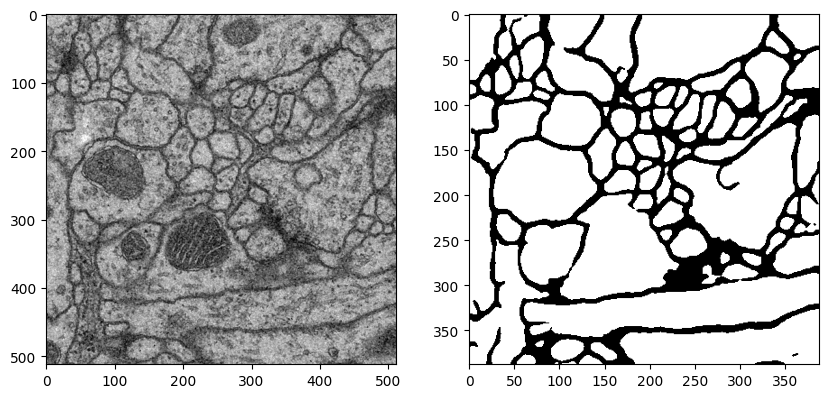
\includegraphics[width=0.7\textwidth]{image/2.png}
    \caption{U-Net模型分割结果}
\end{figure}

\textbf{结果分析:}
\begin{itemize}
    \item U-Net模型对复杂背景的分割效果较好,能够较好地保留细节。
    \item 算法适用于复杂纹理背景,对比度不明显的图像。
    \item U-Net模型的训练时间较长,但分割效果较好。
\end{itemize}

\subsection*{实验结果分析}
\begin{enumerate}
    \item \textbf{传统方法(大津阈值法)}:
    \begin{itemize}
        \item \textbf{优点}:实现简单、计算速度快、对比度明显的图像表现良好。
        \item \textbf{缺点}:对复杂纹理、噪声较多或边界模糊的医学图像效果不佳。在实验中,大津阈值法无法有效区分神经组织边界,导致分割结果不准确。
        \item \textbf{适用场景}:适用于结构清晰、前景和背景对比度大的简单图像分割。
    \end{itemize}

    \item \textbf{深度学习方法(U-Net)}:
    \begin{itemize}
        \item \textbf{优点}:U-Net 对复杂的图像结构具有良好的分割能力,能够捕获全局上下文信息,同时保留细粒度的局部特征。实验中,U-Net 在测试集上的 Dice 系数达到了 0.85,明显优于传统方法。
        \item \textbf{缺点}:训练时间长,对计算资源需求高;对数据量的需求较大,但通过数据增强可以在小样本情况下取得较好的效果。
        \item \textbf{适用场景}:适用于复杂背景、细节丰富的医学图像分割任务。
    \end{itemize}
\end{enumerate}

\subsubsection*{两种方法的异同点}
\begin{table}[h!]
\centering
\begin{tabular}{|l|l|l|}
\hline
\textbf{维度}        & \textbf{传统方法(大津阈值法)}      & \textbf{深度学习方法(U-Net)}      \\ \hline
\textbf{算法原理}    & 基于直方图统计的全局阈值分割方法     & 基于像素分类的卷积神经网络模型       \\ \hline
\textbf{实现复杂度}  & 简单易实现                         & 实现复杂,需要构建模型和训练         \\ \hline
\textbf{计算速度}    & 快,适合实时应用                   & 慢,需训练模型,但推理速度较快        \\ \hline
\textbf{对噪声的鲁棒性} & 对噪声敏感                       & 能够一定程度处理噪声和复杂背景       \\ \hline
\textbf{对数据依赖}  & 无需额外数据支持                   & 需要训练数据,并受数据质量影响        \\ \hline
\textbf{分割效果}    & 适用于对比度明显的简单图像         & 适用于细节复杂的医学图像             \\ \hline
\end{tabular}
\caption{传统方法与深度学习方法的比较}
\end{table}

\subsubsection*{对两种方法异同的理解}
\begin{enumerate}
    \item \textbf{本质区别}:
    \begin{itemize}
        \item 传统方法是基于规则的全局阈值分割,无法适应图像内容的复杂性。
        \item 深度学习方法是基于数据驱动的像素分类,能够学习到图像的语义信息,对细节和复杂场景表现更佳。
    \end{itemize}

    \item \textbf{适用场景}:
    \begin{itemize}
        \item 大津阈值法适合快速处理简单图像,是一种轻量级方案。
        \item U-Net 适用于高精度医学图像分割任务,能处理噪声和复杂背景,但需要更高的计算资源支持。
    \end{itemize}
\end{enumerate} 

\newpage

\begin{thebibliography}{99}

    \bibitem{Schonhoff2007}
    T.A. Schonhoff \& A.A. Giordano, \textit{Detection and Estimation: Theory and its Applications}. Pearson Education, Inc., 2007. (信号检测与估计——理论与应用,关欣等译,电子工业出版社,2012年).
    
    \bibitem{Srinath1996}
    M.D. Srinath, P.K. Rajasekaran \& R. Viswanathan, \textit{Introduction to Statistical Signal Processing with Applications}. Prentice Hall, 1996.  
    
    \bibitem{Kay1993}
    Steven M. Kay, \textit{Fundamentals of Statistical Signal Processing, Volume I: Estimation Theory} (©1993) \& \textit{Volume II: Detection Theory} (©1998). Pearson Education. (《统计信号处理基础:估计与检测理论(卷 I、卷 II合集)》,罗鹏飞等译,电子工业出版社,2023年).  
    
    \bibitem{Candy2016}
    James V. Candy, \textit{Bayesian Signal Processing: Classical, Modern, and Particle Filtering Methods} (2nd ed.). John Wiley \& Sons, Inc., 2016. (宗华等译,哈尔滨工业大学出版社,2023年).  
    
    \bibitem{VanTrees2013}
    Harry L. Van Trees, Kristine L. Bell, with Zhi Tian, \textit{Detection Estimation and Modulation Theory, Part I: Detection, Estimation, and Filtering Theory} (2nd ed.). John Wiley \& Sons, Inc., 2013.  
    
    \bibitem{ChatGPT2024}
    ChatGPT by OpenAI (2024). Personal communication and consultation for generating LaTeX formatting, experimental methodology, and model evaluation strategies. OpenAI, \url{https://www.openai.com}.  
    
\end{thebibliography}
    
    

\end{document}